
% Default to the notebook output style

    


% Inherit from the specified cell style.




    
\documentclass{article}

    
    
    \usepackage{graphicx} % Used to insert images
    \usepackage{adjustbox} % Used to constrain images to a maximum size 
    \usepackage{color} % Allow colors to be defined
    \usepackage{enumerate} % Needed for markdown enumerations to work
    \usepackage{geometry} % Used to adjust the document margins
    \usepackage{amsmath} % Equations
    \usepackage{amssymb} % Equations
    \usepackage{eurosym} % defines \euro
    \usepackage[mathletters]{ucs} % Extended unicode (utf-8) support
    \usepackage[utf8x]{inputenc} % Allow utf-8 characters in the tex document
    \usepackage{fancyvrb} % verbatim replacement that allows latex
    \usepackage{grffile} % extends the file name processing of package graphics 
                         % to support a larger range 
    % The hyperref package gives us a pdf with properly built
    % internal navigation ('pdf bookmarks' for the table of contents,
    % internal cross-reference links, web links for URLs, etc.)
    \usepackage{hyperref}
    \usepackage{longtable} % longtable support required by pandoc >1.10
    \usepackage{booktabs}  % table support for pandoc > 1.12.2
    

    
    
    \definecolor{orange}{cmyk}{0,0.4,0.8,0.2}
    \definecolor{darkorange}{rgb}{.71,0.21,0.01}
    \definecolor{darkgreen}{rgb}{.12,.54,.11}
    \definecolor{myteal}{rgb}{.26, .44, .56}
    \definecolor{gray}{gray}{0.45}
    \definecolor{lightgray}{gray}{.95}
    \definecolor{mediumgray}{gray}{.8}
    \definecolor{inputbackground}{rgb}{.95, .95, .85}
    \definecolor{outputbackground}{rgb}{.95, .95, .95}
    \definecolor{traceback}{rgb}{1, .95, .95}
    % ansi colors
    \definecolor{red}{rgb}{.6,0,0}
    \definecolor{green}{rgb}{0,.65,0}
    \definecolor{brown}{rgb}{0.6,0.6,0}
    \definecolor{blue}{rgb}{0,.145,.698}
    \definecolor{purple}{rgb}{.698,.145,.698}
    \definecolor{cyan}{rgb}{0,.698,.698}
    \definecolor{lightgray}{gray}{0.5}
    
    % bright ansi colors
    \definecolor{darkgray}{gray}{0.25}
    \definecolor{lightred}{rgb}{1.0,0.39,0.28}
    \definecolor{lightgreen}{rgb}{0.48,0.99,0.0}
    \definecolor{lightblue}{rgb}{0.53,0.81,0.92}
    \definecolor{lightpurple}{rgb}{0.87,0.63,0.87}
    \definecolor{lightcyan}{rgb}{0.5,1.0,0.83}
    
    % commands and environments needed by pandoc snippets
    % extracted from the output of `pandoc -s`
    \DefineVerbatimEnvironment{Highlighting}{Verbatim}{commandchars=\\\{\}}
    % Add ',fontsize=\small' for more characters per line
    \newenvironment{Shaded}{}{}
    \newcommand{\KeywordTok}[1]{\textcolor[rgb]{0.00,0.44,0.13}{\textbf{{#1}}}}
    \newcommand{\DataTypeTok}[1]{\textcolor[rgb]{0.56,0.13,0.00}{{#1}}}
    \newcommand{\DecValTok}[1]{\textcolor[rgb]{0.25,0.63,0.44}{{#1}}}
    \newcommand{\BaseNTok}[1]{\textcolor[rgb]{0.25,0.63,0.44}{{#1}}}
    \newcommand{\FloatTok}[1]{\textcolor[rgb]{0.25,0.63,0.44}{{#1}}}
    \newcommand{\CharTok}[1]{\textcolor[rgb]{0.25,0.44,0.63}{{#1}}}
    \newcommand{\StringTok}[1]{\textcolor[rgb]{0.25,0.44,0.63}{{#1}}}
    \newcommand{\CommentTok}[1]{\textcolor[rgb]{0.38,0.63,0.69}{\textit{{#1}}}}
    \newcommand{\OtherTok}[1]{\textcolor[rgb]{0.00,0.44,0.13}{{#1}}}
    \newcommand{\AlertTok}[1]{\textcolor[rgb]{1.00,0.00,0.00}{\textbf{{#1}}}}
    \newcommand{\FunctionTok}[1]{\textcolor[rgb]{0.02,0.16,0.49}{{#1}}}
    \newcommand{\RegionMarkerTok}[1]{{#1}}
    \newcommand{\ErrorTok}[1]{\textcolor[rgb]{1.00,0.00,0.00}{\textbf{{#1}}}}
    \newcommand{\NormalTok}[1]{{#1}}
    
    % Define a nice break command that doesn't care if a line doesn't already
    % exist.
    \def\br{\hspace*{\fill} \\* }
    % Math Jax compatability definitions
    \def\gt{>}
    \def\lt{<}
    % Document parameters
    \title{STA663\ Final\ Project}
    \author{John Pura}
    
    
    

    % Pygments definitions
    
\makeatletter
\def\PY@reset{\let\PY@it=\relax \let\PY@bf=\relax%
    \let\PY@ul=\relax \let\PY@tc=\relax%
    \let\PY@bc=\relax \let\PY@ff=\relax}
\def\PY@tok#1{\csname PY@tok@#1\endcsname}
\def\PY@toks#1+{\ifx\relax#1\empty\else%
    \PY@tok{#1}\expandafter\PY@toks\fi}
\def\PY@do#1{\PY@bc{\PY@tc{\PY@ul{%
    \PY@it{\PY@bf{\PY@ff{#1}}}}}}}
\def\PY#1#2{\PY@reset\PY@toks#1+\relax+\PY@do{#2}}

\expandafter\def\csname PY@tok@gd\endcsname{\def\PY@tc##1{\textcolor[rgb]{0.63,0.00,0.00}{##1}}}
\expandafter\def\csname PY@tok@gu\endcsname{\let\PY@bf=\textbf\def\PY@tc##1{\textcolor[rgb]{0.50,0.00,0.50}{##1}}}
\expandafter\def\csname PY@tok@gt\endcsname{\def\PY@tc##1{\textcolor[rgb]{0.00,0.27,0.87}{##1}}}
\expandafter\def\csname PY@tok@gs\endcsname{\let\PY@bf=\textbf}
\expandafter\def\csname PY@tok@gr\endcsname{\def\PY@tc##1{\textcolor[rgb]{1.00,0.00,0.00}{##1}}}
\expandafter\def\csname PY@tok@cm\endcsname{\let\PY@it=\textit\def\PY@tc##1{\textcolor[rgb]{0.25,0.50,0.50}{##1}}}
\expandafter\def\csname PY@tok@vg\endcsname{\def\PY@tc##1{\textcolor[rgb]{0.10,0.09,0.49}{##1}}}
\expandafter\def\csname PY@tok@m\endcsname{\def\PY@tc##1{\textcolor[rgb]{0.40,0.40,0.40}{##1}}}
\expandafter\def\csname PY@tok@mh\endcsname{\def\PY@tc##1{\textcolor[rgb]{0.40,0.40,0.40}{##1}}}
\expandafter\def\csname PY@tok@go\endcsname{\def\PY@tc##1{\textcolor[rgb]{0.53,0.53,0.53}{##1}}}
\expandafter\def\csname PY@tok@ge\endcsname{\let\PY@it=\textit}
\expandafter\def\csname PY@tok@vc\endcsname{\def\PY@tc##1{\textcolor[rgb]{0.10,0.09,0.49}{##1}}}
\expandafter\def\csname PY@tok@il\endcsname{\def\PY@tc##1{\textcolor[rgb]{0.40,0.40,0.40}{##1}}}
\expandafter\def\csname PY@tok@cs\endcsname{\let\PY@it=\textit\def\PY@tc##1{\textcolor[rgb]{0.25,0.50,0.50}{##1}}}
\expandafter\def\csname PY@tok@cp\endcsname{\def\PY@tc##1{\textcolor[rgb]{0.74,0.48,0.00}{##1}}}
\expandafter\def\csname PY@tok@gi\endcsname{\def\PY@tc##1{\textcolor[rgb]{0.00,0.63,0.00}{##1}}}
\expandafter\def\csname PY@tok@gh\endcsname{\let\PY@bf=\textbf\def\PY@tc##1{\textcolor[rgb]{0.00,0.00,0.50}{##1}}}
\expandafter\def\csname PY@tok@ni\endcsname{\let\PY@bf=\textbf\def\PY@tc##1{\textcolor[rgb]{0.60,0.60,0.60}{##1}}}
\expandafter\def\csname PY@tok@nl\endcsname{\def\PY@tc##1{\textcolor[rgb]{0.63,0.63,0.00}{##1}}}
\expandafter\def\csname PY@tok@nn\endcsname{\let\PY@bf=\textbf\def\PY@tc##1{\textcolor[rgb]{0.00,0.00,1.00}{##1}}}
\expandafter\def\csname PY@tok@no\endcsname{\def\PY@tc##1{\textcolor[rgb]{0.53,0.00,0.00}{##1}}}
\expandafter\def\csname PY@tok@na\endcsname{\def\PY@tc##1{\textcolor[rgb]{0.49,0.56,0.16}{##1}}}
\expandafter\def\csname PY@tok@nb\endcsname{\def\PY@tc##1{\textcolor[rgb]{0.00,0.50,0.00}{##1}}}
\expandafter\def\csname PY@tok@nc\endcsname{\let\PY@bf=\textbf\def\PY@tc##1{\textcolor[rgb]{0.00,0.00,1.00}{##1}}}
\expandafter\def\csname PY@tok@nd\endcsname{\def\PY@tc##1{\textcolor[rgb]{0.67,0.13,1.00}{##1}}}
\expandafter\def\csname PY@tok@ne\endcsname{\let\PY@bf=\textbf\def\PY@tc##1{\textcolor[rgb]{0.82,0.25,0.23}{##1}}}
\expandafter\def\csname PY@tok@nf\endcsname{\def\PY@tc##1{\textcolor[rgb]{0.00,0.00,1.00}{##1}}}
\expandafter\def\csname PY@tok@si\endcsname{\let\PY@bf=\textbf\def\PY@tc##1{\textcolor[rgb]{0.73,0.40,0.53}{##1}}}
\expandafter\def\csname PY@tok@s2\endcsname{\def\PY@tc##1{\textcolor[rgb]{0.73,0.13,0.13}{##1}}}
\expandafter\def\csname PY@tok@vi\endcsname{\def\PY@tc##1{\textcolor[rgb]{0.10,0.09,0.49}{##1}}}
\expandafter\def\csname PY@tok@nt\endcsname{\let\PY@bf=\textbf\def\PY@tc##1{\textcolor[rgb]{0.00,0.50,0.00}{##1}}}
\expandafter\def\csname PY@tok@nv\endcsname{\def\PY@tc##1{\textcolor[rgb]{0.10,0.09,0.49}{##1}}}
\expandafter\def\csname PY@tok@s1\endcsname{\def\PY@tc##1{\textcolor[rgb]{0.73,0.13,0.13}{##1}}}
\expandafter\def\csname PY@tok@sh\endcsname{\def\PY@tc##1{\textcolor[rgb]{0.73,0.13,0.13}{##1}}}
\expandafter\def\csname PY@tok@sc\endcsname{\def\PY@tc##1{\textcolor[rgb]{0.73,0.13,0.13}{##1}}}
\expandafter\def\csname PY@tok@sx\endcsname{\def\PY@tc##1{\textcolor[rgb]{0.00,0.50,0.00}{##1}}}
\expandafter\def\csname PY@tok@bp\endcsname{\def\PY@tc##1{\textcolor[rgb]{0.00,0.50,0.00}{##1}}}
\expandafter\def\csname PY@tok@c1\endcsname{\let\PY@it=\textit\def\PY@tc##1{\textcolor[rgb]{0.25,0.50,0.50}{##1}}}
\expandafter\def\csname PY@tok@kc\endcsname{\let\PY@bf=\textbf\def\PY@tc##1{\textcolor[rgb]{0.00,0.50,0.00}{##1}}}
\expandafter\def\csname PY@tok@c\endcsname{\let\PY@it=\textit\def\PY@tc##1{\textcolor[rgb]{0.25,0.50,0.50}{##1}}}
\expandafter\def\csname PY@tok@mf\endcsname{\def\PY@tc##1{\textcolor[rgb]{0.40,0.40,0.40}{##1}}}
\expandafter\def\csname PY@tok@err\endcsname{\def\PY@bc##1{\setlength{\fboxsep}{0pt}\fcolorbox[rgb]{1.00,0.00,0.00}{1,1,1}{\strut ##1}}}
\expandafter\def\csname PY@tok@kd\endcsname{\let\PY@bf=\textbf\def\PY@tc##1{\textcolor[rgb]{0.00,0.50,0.00}{##1}}}
\expandafter\def\csname PY@tok@ss\endcsname{\def\PY@tc##1{\textcolor[rgb]{0.10,0.09,0.49}{##1}}}
\expandafter\def\csname PY@tok@sr\endcsname{\def\PY@tc##1{\textcolor[rgb]{0.73,0.40,0.53}{##1}}}
\expandafter\def\csname PY@tok@mo\endcsname{\def\PY@tc##1{\textcolor[rgb]{0.40,0.40,0.40}{##1}}}
\expandafter\def\csname PY@tok@kn\endcsname{\let\PY@bf=\textbf\def\PY@tc##1{\textcolor[rgb]{0.00,0.50,0.00}{##1}}}
\expandafter\def\csname PY@tok@mi\endcsname{\def\PY@tc##1{\textcolor[rgb]{0.40,0.40,0.40}{##1}}}
\expandafter\def\csname PY@tok@gp\endcsname{\let\PY@bf=\textbf\def\PY@tc##1{\textcolor[rgb]{0.00,0.00,0.50}{##1}}}
\expandafter\def\csname PY@tok@o\endcsname{\def\PY@tc##1{\textcolor[rgb]{0.40,0.40,0.40}{##1}}}
\expandafter\def\csname PY@tok@kr\endcsname{\let\PY@bf=\textbf\def\PY@tc##1{\textcolor[rgb]{0.00,0.50,0.00}{##1}}}
\expandafter\def\csname PY@tok@s\endcsname{\def\PY@tc##1{\textcolor[rgb]{0.73,0.13,0.13}{##1}}}
\expandafter\def\csname PY@tok@kp\endcsname{\def\PY@tc##1{\textcolor[rgb]{0.00,0.50,0.00}{##1}}}
\expandafter\def\csname PY@tok@w\endcsname{\def\PY@tc##1{\textcolor[rgb]{0.73,0.73,0.73}{##1}}}
\expandafter\def\csname PY@tok@kt\endcsname{\def\PY@tc##1{\textcolor[rgb]{0.69,0.00,0.25}{##1}}}
\expandafter\def\csname PY@tok@ow\endcsname{\let\PY@bf=\textbf\def\PY@tc##1{\textcolor[rgb]{0.67,0.13,1.00}{##1}}}
\expandafter\def\csname PY@tok@sb\endcsname{\def\PY@tc##1{\textcolor[rgb]{0.73,0.13,0.13}{##1}}}
\expandafter\def\csname PY@tok@k\endcsname{\let\PY@bf=\textbf\def\PY@tc##1{\textcolor[rgb]{0.00,0.50,0.00}{##1}}}
\expandafter\def\csname PY@tok@se\endcsname{\let\PY@bf=\textbf\def\PY@tc##1{\textcolor[rgb]{0.73,0.40,0.13}{##1}}}
\expandafter\def\csname PY@tok@sd\endcsname{\let\PY@it=\textit\def\PY@tc##1{\textcolor[rgb]{0.73,0.13,0.13}{##1}}}

\def\PYZbs{\char`\\}
\def\PYZus{\char`\_}
\def\PYZob{\char`\{}
\def\PYZcb{\char`\}}
\def\PYZca{\char`\^}
\def\PYZam{\char`\&}
\def\PYZlt{\char`\<}
\def\PYZgt{\char`\>}
\def\PYZsh{\char`\#}
\def\PYZpc{\char`\%}
\def\PYZdl{\char`\$}
\def\PYZhy{\char`\-}
\def\PYZsq{\char`\'}
\def\PYZdq{\char`\"}
\def\PYZti{\char`\~}
% for compatibility with earlier versions
\def\PYZat{@}
\def\PYZlb{[}
\def\PYZrb{]}
\makeatother


    % Exact colors from NB
    \definecolor{incolor}{rgb}{0.0, 0.0, 0.5}
    \definecolor{outcolor}{rgb}{0.545, 0.0, 0.0}



    
    % Prevent overflowing lines due to hard-to-break entities
    \sloppy 
    % Setup hyperref package
    \hypersetup{
      breaklinks=true,  % so long urls are correctly broken across lines
      colorlinks=true,
      urlcolor=blue,
      linkcolor=darkorange,
      citecolor=darkgreen,
      }
    % Slightly bigger margins than the latex defaults
    
    \geometry{verbose,tmargin=1in,bmargin=1in,lmargin=1in,rmargin=1in}
    
    

    \begin{document}
    
    
    \maketitle
    
    

    
    \section{Introduction}\label{introduction}

    Estimating sparse precision matrices is an important problem in various
statistical areas, such as principal component analysis and graphical
models. For example, under Gaussian graphical models, estimating the
support of the precision matrix allows one to recover the conditional
dependence between components of a graph. Precision matrix estimation is
generally computationally expensive, which is further exarcerbated by
high-dimensional settings, particularly when the number of parameters,
$p$, exceeds the sample size, $n$. Several algorithms have been
developed in recent years to address these issues. The goal of this
project is to implement one such algorithm - the constrained ℓ1
minimization estimator (CLIME), which is an efficient and accurate tool
in estimating sparse precision matrices (Cai, et al., 2011).

This project implements a fast version of CLIME using the parametric
simplex method (PSM) (Vanderbei, 2008; Pang, et al., 2014). A Python
implementation would enhance efficiency and scalability compared to the
existing \texttt{R} package \texttt{fastclime}. Additionally, the code
leverages existing C code for the PSM linear programming (LP) solver to
further speed up performance.

In the following report, I present a stable, well-tested version of
\texttt{fastclime} in Python. Results include numerical benchmarking
under simulated data and comparison to existing state-of-the-art
algorithms that solve a similar family of problems in precision matrix
estimation. The Python implementation of \texttt{fastclime} performs
comparably to the \texttt{R} version in terms of speed when tested
against a wide range of data with fixed sample size and varying number
of predictors. Additionally, \texttt{fastclime} results are favorable
compared to existing algorithms for precision matrix estimation. A
section on ongoing/future work extends the CLIME estimation problem to
the case when covariates are involved.

    \section{CLIME method}\label{clime-method}

    Let $\textbf{x}=(x_1,...,x_n)\in\mathbb{R}^{nxp}$ be $n$ observations of
a $p$-dimensional random vector $\textbf{X}=(X_1,...,X_p)^T$. For the
$n\times p$ data matrix, $\textbf{x}$, or its corresponding $p\times p$
sample covariance matrix,
$\Sigma_n=\frac{1}{n}\sum_{k=1}^{n}(x_k-\bar{x})(x_k-\bar{x})^T$, the
CLIME method solves the following optimization problem:

\begin{equation*}
\hat{\Omega}=\arg_\Omega\min \| \mathbf{\Omega} \|_1\text{ subject to }\|\mathbf{\Sigma}_n\mathbf{\Omega}-\textbf{I}\|_\infty\le\lambda_n\text{, }\mathbf{\Omega}\in\mathbb{R}^{p\times p}
\end{equation*}

where $\hat{\Omega}$ is the estimated precision matrix and $\lambda_n$
is a tuning parameter.

This minimization problem can be further decomposed into $p$ smaller
problems, allowing us to recover the precision matrix in a column by
column fashion (i.e.~solving $p$ optimization problems).

\begin{equation}
\hat{\omega}_i=\arg_\omega\min | \mathbf{\omega} |_1\text{ subject to }|\mathbf{\Sigma}_n\mathbf{\omega}-\textbf{e}_i|_\infty\le\lambda_n\text{, }\mathbf{\omega}\in\mathbb{R}^{p}
\end{equation}

where $\textbf{e}_i$ is the standard basis vector.

    \subsection{Parametric Simplex Method}\label{parametric-simplex-method}

    The simplex method is a linear programming method that can be used to
solve the following constrained problem:

\begin{equation*}
\max c^T x \text{ subject to } Ax\le b, \quad x\ge 0
\end{equation*}

where $A\in\mathbb{R}^{n\times d}$, $c\in\mathbb{R}^d$, and
$b\in\mathbb{R}^n$.

The parametric simplex method (PSM) is an alternative formulation of the
simplex method with the following rule:

\begin{equation}
\max (c+\lambda c^{*})^T x \text{ subject to } Ax\le b + \lambda b^{*}, \quad x\ge 0 
\end{equation}

where A, b, and c are the same as above and $b^{*}\ge 0$ and
$c^{*}\le 0$ are perturbation vectors.

Here, $\lambda$ is related to the tuning parameter above in the CLIME
problem. The PSM algorithm performs pivots to reduce $\lambda$ until the
optimal solution is reached (when $\lambda = 0$). Therefore, by
reformulating (1) as (3) the entire solution path for the original CLIME
problem can be determined from the solution path of a single regularized
LP problem using PSM. The optimal solution is achieved in only a few
iterations.

    \subsection{CLIME Pseudocode}\label{clime-pseudocode}

    \begin{enumerate}
\def\labelenumi{\arabic{enumi}.}
\item
  Normalize data, $\textbf{x}$, to have zero mean and unit standard
  deviation along each column.
\item
  Estimate empirical covariance matrix,
  $\Sigma_n=\frac{n-1}{n}\textbf{X}\textbf{X}^T$, where $\textbf{X}$ is
  the normalized data.
\item
  Initialize $\lambda_{min}$ and path length size.
\item
  For $1\le i\le p\text{ columns}$: Reformulate the CLIME problem to use
  PSM:
\end{enumerate}

\[\hat{\omega}_i^1\leftarrow\arg_{{\omega}_i}\min (\mathbf{\omega^{+}-\omega^{-}}) \text{ subject to  } \left( \begin{array}{cc}
\Sigma_n & -\Sigma_n \\
-\Sigma_n & \Sigma_n \end{array} \right) 
\left( \begin{array}{c}
\omega^+\\
\omega^-\end{array} \right)\le\left( \begin{array}{c}
\lambda+e_i\\
\lambda-e_i\end{array} \right)\]

where $\omega=\omega^{+}-\omega^-$ and
$\|\omega\|_1=\omega^{+}+\omega^-$, $\omega^{+}\ge 0, \omega^{-}\ge 0$.

Comparing above to $(1)$ and $(2)$,
$A = \left( \begin{array}{cc} \Sigma_n & -\Sigma_n \\ -\Sigma_n & \Sigma_n \end{array} \right)$,
$b=\left( \begin{array}{c} e_i\\ -e_i\end{array} \right)$,
$c=\textbf{-1}^T$, $b^{*}=\textbf{1}^T$, and $c^{*}=\textbf{0}^T$

\begin{enumerate}
\def\labelenumi{\arabic{enumi}.}
\setcounter{enumi}{4}
\itemsep1pt\parskip0pt\parsep0pt
\item
  Symmetrize
  $\hat{\Omega}=(\hat{\omega}_{ij})=(\hat{\omega}_{ji})\leftarrow\omega^1_{ij}I\{|\hat{\omega}_{ij}^1|\le|\hat{\omega}_{ji}^1|\}+\omega^1_{ji}I\{|\hat{\omega}_{ij}^1|\gt|\hat{\omega}_{ji}^1|\}$
\end{enumerate}

    \subsection{Python Implementation}\label{python-implementation}

    Using Python/C API, I wrapped the \texttt{parametric.c} function from
the \texttt{src} directory of the \texttt{fastclime} \texttt{R} package
and imported it as its own module in Python for solving LP problems. All
other functions are implemented using the \texttt{Numpy} package in
Python.

I also included several functions not found in the original
\texttt{fastclime} \texttt{R} package. Specifically, I have implemented
regularization parameter selection, which is important in estimation of
both precision matrices and high-dimensional undirected graphs. The
regularization parameter, $\lambda$ is important in controlling the
sparsity of the graph. Therefore its choice is critical in maintaining
valid statistical inferences regarding the conditional independence
between nodes or features in the graph. I considered popular metrics,
such as the Akaike Information Criterion (AIC) and Bayesian Information
Criterion (BIC).

    \section{Numerical Results}\label{numerical-results}

    \subsection{Unit Tests}\label{unit-tests}

    Unit tests were performed to verify correctness of the Python
implementation subject to various inputs. Each function, if possible,
was subjected to several inputs and tested to produce the correct value
or an exception error. All tests are documented in the file
\texttt{test\_fastclime.py}. As seen below, all tests passed, suggesting
correct functionality of \texttt{fastclime} in Python.

    \begin{Verbatim}[commandchars=\\\{\}]
{\color{incolor}In [{\color{incolor}1}]:} \PY{o}{!} py.test
\end{Verbatim}

    \begin{Verbatim}[commandchars=\\\{\}]
============================= test session starts ==============================
platform linux2 -- Python 2.7.9 -- py-1.4.25 -- pytest-2.6.3
collected 21 items 

test\_fastclime.py {\ldots}

{\color{green}}========================== 21 passed in 3.22 seconds ===========================
    \end{Verbatim}

    \subsection{Profiling}\label{profiling}

    The line profiler in Python was used to identify areas of bottleneck
within the integrated functions, \texttt{fastclime\_R} and
\texttt{fastclime\_est\_select}. The profiling code is located in the
file \texttt{Profiling.ipynb}. In both situations, over 90\% of the
runtime was due to the \texttt{parametric.mainfunc} function in the
\texttt{parametric} module. This scenario is optimal as this module is
purely compiled in C, which provides a fast, efficient way of running
the PSM solver.

    \subsection{Numerical Simulations}\label{numerical-simulations}

    \subsubsection{Benchmarking Python and
R}\label{benchmarking-python-and-r}

    First I benchmarked performance times of the Python and \texttt{R}
implementations of \texttt{fastclime} for a sparse random graph with
varying number of predictors and fixed sample size, $n=200$. Using the
\texttt{timeit} module, the runtime was estimated for predictor sizes
$p=50, 100, 200, 400, \text{and } 800$. For the purposes of this
project, only one instance of the function was timed. As seen in Table 1
below, the times (in seconds) are comparable between Python and R. Any
speedboost to the Python program would potentially require coding the
entire suite of functions in C.

    \begin{Verbatim}[commandchars=\\\{\}]
{\color{incolor}In [{\color{incolor}2}]:} \PY{k+kn}{import} \PY{n+nn}{pandas} \PY{k+kn}{as} \PY{n+nn}{pd}
        \PY{k}{print} \PY{l+s}{\PYZdq{}}\PY{l+s}{Table 1. Timing performance of fastclime implementations in Python and R in seconds}\PY{l+s}{\PYZdq{}}
        \PY{k}{print} \PY{n}{pd}\PY{o}{.}\PY{n}{read\PYZus{}csv}\PY{p}{(}\PY{l+s}{\PYZdq{}}\PY{l+s}{benchmark.csv}\PY{l+s}{\PYZdq{}}\PY{p}{,} \PY{n}{sep}\PY{o}{=}\PY{l+s}{\PYZsq{}}\PY{l+s}{,}\PY{l+s}{\PYZsq{}}\PY{p}{,} \PY{n}{skipinitialspace}\PY{o}{=}\PY{n+nb+bp}{False}\PY{p}{)}
\end{Verbatim}

    \begin{Verbatim}[commandchars=\\\{\}]
Table 1. Timing performance of fastclime implementations in Python and R in seconds
        p    50   100   200    400     800
   Python  0.04  0.33  4.37  32.97  237.96
        R  0.18  0.46  4.82  33.04  241.79
    \end{Verbatim}

    \subsubsection{Comparison with existing algorithms for precision matrix
estimation}\label{comparison-with-existing-algorithms-for-precision-matrix-estimation}

    \texttt{TIGER} is a tuning insensitive graph estimation and regression
procedure that is implemented in the \texttt{flare} package in
\texttt{R} (original paper: Liu and Wang, 2012, R package: Li, et al.,
2013). It is closely related to the SQRT-Lasso and solves the following
problem:

\begin{equation}
\min \|X − XB\|_{2,1} + \lambda\|B\|_1 \text{ subject to } B_{jj} = 0
\end{equation}

where $\|\cdot\|_{2,1}$ is the $L_{2,1}$ norm.

One advantage of \texttt{TIGER} over other regularization methods, is
that it does not require a model selection procedure like
\texttt{fastclime} for selecting the regularization parameter. Instead
the user manually selects the parameter to be $\sqrt{\frac{\log p}{n}}$,
which is theoretically consistent and does not depend on unknown
quantities.

    To determine the efficiency of these two methods, a single run was
performed for each method, for fixed $n=100$ and varying
$p=100,200,300,400$.

    \begin{Verbatim}[commandchars=\\\{\}]
{\color{incolor}In [{\color{incolor}3}]:} \PY{k+kn}{import} \PY{n+nn}{pandas} \PY{k+kn}{as} \PY{n+nn}{pd}
        \PY{k}{print} \PY{l+s}{\PYZdq{}}\PY{l+s}{Table 2. Timing performance of fastclime and TIGER solvers in seconds}\PY{l+s}{\PYZdq{}}
        \PY{k}{print} \PY{n}{pd}\PY{o}{.}\PY{n}{read\PYZus{}csv}\PY{p}{(}\PY{l+s}{\PYZdq{}}\PY{l+s}{tigerfc.csv}\PY{l+s}{\PYZdq{}}\PY{p}{,} \PY{n}{sep}\PY{o}{=}\PY{l+s}{\PYZsq{}}\PY{l+s}{,}\PY{l+s}{\PYZsq{}}\PY{p}{,} \PY{n}{skipinitialspace}\PY{o}{=}\PY{n+nb+bp}{False}\PY{p}{)}
\end{Verbatim}

    \begin{Verbatim}[commandchars=\\\{\}]
Table 2. Timing performance of fastclime and TIGER solvers in seconds
           p   100   200    300    400
   fastclime  0.72  4.70  14.20  31.06
       TIGER  0.86  2.76   5.83  11.83
    \end{Verbatim}

    From the table above, it seems that \texttt{TIGER} outperforms
\texttt{fastclime} in terms of efficiency. This is likely due to the
slightly less complex formulation of \texttt{TIGER}. However, more runs
would be needed to confirm this observation.

    I then considered two simulated models of the sparse precision matrix.

The first model considers a banded precision matrix, such that
$\Omega_0={\omega^0_{ij}}=\mathbb{I}\{1\le|i-j|\le10\}$.

The second model considers a random, sparse precision matrix, such that
$\Omega_0={\omega^0_{ij}}={\omega^0_{ji}}=1\text{ for }i\neq j\text{ with pr. } 0.05\text{ and zero otherwise}$.

The BIC metric was used in \texttt{fastclime\_select} to obtain the
optimal regularization parameter and corresponding precision matrix.
Default settings were used in \texttt{flare}, with the exception of
precision, which was set to 1e-5.

    
\begin{figure}[!H]
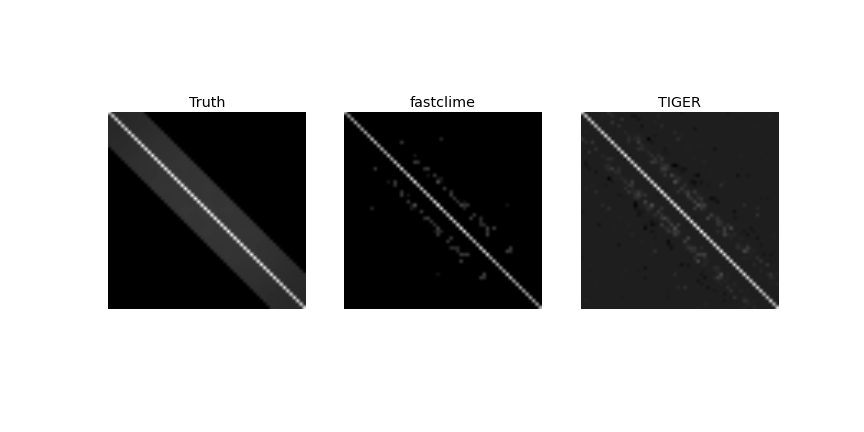
\includegraphics[width=\linewidth]{banded.png}
\caption {Simulation results for banded precision matrix, n = 200, p = 60}
\label{fig:banded}
\end{figure}

\begin{figure}[!H]
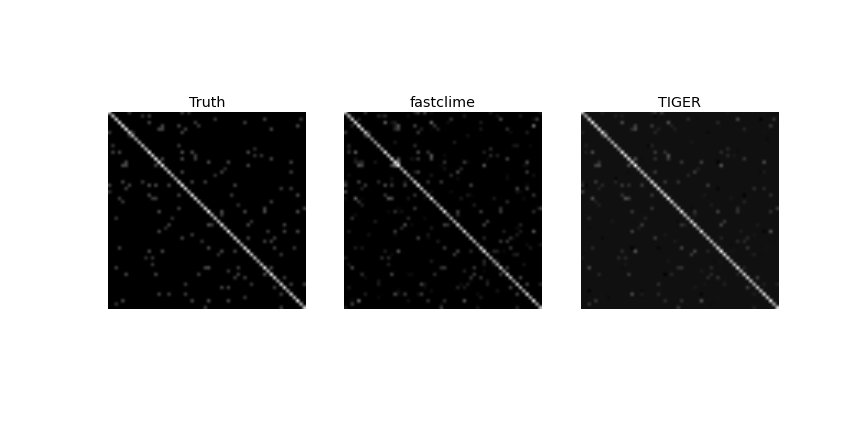
\includegraphics[width=\linewidth]{random.png}
\caption {Simulation results for random precision matrix, n = 200, p = 60}
\label{fig:random}
\end{figure}     

    Figures 1 and 2 show heatmaps of the recovered precision matrices. Black
pixels represent zeros identified in the estimation. In the banded
model, \texttt{fastclime} tended to recover less of the off-diagonal
elements along the band. The estimate from \texttt{TIGER} also shows
stronger intensities along the main diagonal, which is consistent with
the true model. In the random graph, the sparsity patterns recovered by
\texttt{fastclime} and \texttt{TIGER} are approximately the same as the
that of the ground truth. However, caution should be taken in
interpreting these graphs, as these only represent a single run for each
of the solvers. A better alternative would be to examine the averaged
heatmap over several runs for each solver.

    Next the accuracy of \texttt{fastclime} and \texttt{TIGER} estimates
with respect to the true precision matrix is quantified for several
models of the true precision matrix. The random precision matrix
structure is considered for fixed $n=200$ and varying
$p=100,200, \text{ and } 300$. Accuracy is quantified using several
matrix norms: infinity (or sup), Frobenius, and $L_2$ norms.

    \begin{Verbatim}[commandchars=\\\{\}]
{\color{incolor}In [{\color{incolor}4}]:} \PY{k+kn}{import} \PY{n+nn}{pandas} \PY{k+kn}{as} \PY{n+nn}{pd}
        \PY{n}{df} \PY{o}{=} \PY{n}{pd}\PY{o}{.}\PY{n}{read\PYZus{}csv}\PY{p}{(}\PY{l+s}{\PYZdq{}}\PY{l+s}{normerrors.csv}\PY{l+s}{\PYZdq{}}\PY{p}{,} \PY{n}{sep}\PY{o}{=}\PY{l+s}{\PYZsq{}}\PY{l+s}{,}\PY{l+s}{\PYZsq{}}\PY{p}{,} \PY{n}{skipinitialspace}\PY{o}{=}\PY{n+nb+bp}{True}\PY{p}{)}
        \PY{k}{print} \PY{l+s}{\PYZdq{}}\PY{l+s}{Table 3a. Absolute errors for fastclime estimate of precision matrix}\PY{l+s}{\PYZdq{}}
        \PY{k}{print} \PY{n}{df}\PY{o}{.}\PY{n}{pivot}\PY{p}{(}\PY{n}{index}\PY{o}{=}\PY{l+s}{\PYZsq{}}\PY{l+s}{Norm}\PY{l+s}{\PYZsq{}}\PY{p}{,} \PY{n}{columns}\PY{o}{=}\PY{l+s}{\PYZsq{}}\PY{l+s}{p}\PY{l+s}{\PYZsq{}}\PY{p}{,} \PY{n}{values}\PY{o}{=}\PY{l+s}{\PYZsq{}}\PY{l+s}{fastclime}\PY{l+s}{\PYZsq{}}\PY{p}{)}
        \PY{k}{print}
        \PY{k}{print} \PY{l+s}{\PYZdq{}}\PY{l+s}{Table 3b. Absolute errors for TIGER estimate of precision matrix}\PY{l+s}{\PYZdq{}}
        \PY{k}{print} \PY{n}{df}\PY{o}{.}\PY{n}{pivot}\PY{p}{(}\PY{n}{index}\PY{o}{=}\PY{l+s}{\PYZsq{}}\PY{l+s}{Norm}\PY{l+s}{\PYZsq{}}\PY{p}{,} \PY{n}{columns}\PY{o}{=}\PY{l+s}{\PYZsq{}}\PY{l+s}{p}\PY{l+s}{\PYZsq{}}\PY{p}{,} \PY{n}{values}\PY{o}{=}\PY{l+s}{\PYZsq{}}\PY{l+s}{TIGER}\PY{l+s}{\PYZsq{}}\PY{p}{)}
\end{Verbatim}

    \begin{Verbatim}[commandchars=\\\{\}]
Table 3a. Absolute errors for fastclime estimate of precision matrix
p            100    200    300    400
Norm                                 
Frobenius  29.28  33.51  85.35  73.23
Infinity   23.91  23.35  50.09  31.32
L2         10.97  12.12  46.68  24.42

Table 3b. Absolute errors for TIGER estimate of precision matrix
p           100   200   300   400
Norm                             
Frobenius  4.93  6.78  7.93  9.81
Infinity   2.39  3.08  2.91  3.42
L2         1.37  1.35  1.26  1.57
    \end{Verbatim}

    Overall, the normed differences between the true and estimate precision
matrices were lowest for \texttt{TIGER}. The Frobenius norm yielded the
largest differences, while the $L_2$ norm yielded the lowest. As
expected, BIC was not a good metric for selecting the optimal
regularization solution for $p > n$ under \texttt{fastclime}. On the
other hand, errors for \texttt{TIGER} were roughly consistent across
varying predictor levels. One can potentially improve on the estimation
errors for the \texttt{fastclime} method through the use of a more
robust metric in the regularization selection.

    \section{Future Work}\label{future-work}

    I am currently in the process of extending CLIME to the estimation of
precision matrices under covariate adjustment, also known as CAPME
(Covariate-adjustmed precision matrix estimation) (Cai, et al., 2013).
This will be a Python implementation of the current \texttt{R} package
\texttt{capme}. The current \texttt{R} package uses different LP solvers
and is generally slow. For comparison, the \texttt{fastclime} package in
\texttt{R} provides results for a $200\times 800$ matrix in under 7
minutes, while the \texttt{clime} package (used in \texttt{capme})
cannot produce results in an hour. Therefore, it would be advantageous,
speed-wise, to implement \texttt{capme} in Python. So far, I have
modified the \texttt{parametric.c} source code (\texttt{parametric2.c})
to leverage PSM and elements of \texttt{fastclime} and provide a
dramatic speed-up compared to \texttt{R}.

    \subsection{CAPME problem}\label{capme-problem}

    Consider the following regression model with covariates:

\[
\textbf{y}=\textbf{x}\Gamma_0^T+\textbf{z}
\]

where $\textbf{y}\in\mathbb{R}^{n\times p}$ is a collection of random
vectors of responses, $\textbf{x}\in\mathbb{R}^{n\times q}$ is a
collection of random vectors of covariates or features, $\Gamma_0$ is an
unknown $p\times q$ coefficient matrix, $\textbf{z}$ is a $n\times p$
normal random vector with mean zero, covariance
$\Sigma_0\in\mathbb{R}^{p\times p}$ and precision matrix
$\Omega_0=\Sigma_0^{-1}$. Assume $\textbf{x}$ and $\textbf{z}$ are
independent and that we have $n$ $iid$ observations
$(\textbf{x}_k,\textbf{y}_k)$, ($k=1,...,n$) for the model.

Using ℓ1 regularization (e.g.~LASSO), we first estimate the coefficient
matrix $\Gamma_0$. Then we estimate $\Omega_0$ using CLIME above. Like
before, we can estimate both $\Gamma_0$ and $\Omega_0$ by performing the
optimization on each column separately.

In order leverage the previously created \texttt{fastclime} module, both estimation
stages were reformulated to the LP form used in PSM. The following
pseudocode illustrates this reparametrization:

    \begin{enumerate}
\def\labelenumi{\arabic{enumi}.}
\item
  Normalize $\textbf{x}$ and $\textbf{y}$ to have zero mean and unit
  standard deviation along each column.
\item
  Compute the sample covariances
  $S_{xy}=\frac{n-1}{n}\mathbb{E}\textbf{XY}^T$ and
  $S_{xx}=\frac{n-1}{n}\mathbb{E}\textbf{XX}^T$, where $\textbf{X}$ and
  $\textbf{Y}$ are the normalized data.
\item
  For $1\le i\le p\text{ columns}$

  Estimate

  \begin{equation}
  \hat{\gamma}_i\leftarrow\arg_{\gamma_i}\min |\gamma_i|_1\text{ subject to }|S_{xy,i}-\gamma_i^T S_{xx}|_\infty \le \lambda_n \quad\quad 
  \end{equation}

  $\text{where }\hat{\Gamma}=(\hat{\gamma}_1,...,\hat{\gamma}_p)^T$ This
  can be reformulated as follows:
  \[\hat{\gamma}_i^1\leftarrow\arg_{{\gamma}_i}\min (\mathbf{\gamma^{+}-\gamma^{-}}) \text{ subject to  } \left( \begin{array}{cc}
  S_{xx} & -S_{xx} \\
  -S_{xx} & S_{xx} \end{array} \right) 
  \left( \begin{array}{c}
  \gamma^+\\
  \gamma^-\end{array} \right)\le\left( \begin{array}{c}
  \lambda+S_{xy,i}\\
  \lambda-S_{xy,i}\end{array} \right)\] where
  $\gamma=\gamma^{+}-\gamma^-$ and $\|\gamma\|_1=\gamma^{+}+\gamma^-$,
  $\gamma^{+}\ge 0, \gamma^{-}\ge 0$. Comparing above to $(2)$ and $(4)$,
  $A = \left( \begin{array}{cc} S_{xx} & -S_{xx} \\ -S_{xx} & S_{xx} \end{array} \right)$,
  $b=\left( \begin{array}{c} S_{xy,i}\\ -S_{xy,i}\end{array} \right)$,
  $c=\textbf{-1}^T$, $b^{*}=\textbf{1}^T$, and $c^{*}=\textbf{0}^T$
\item
  Substitute the estimated $\hat{\Gamma}$ in $(4)$ and compute the
  sample covariance, $S_{yy}$, substituting the column means with
  $\hat{\Gamma} x_k$, $1\le k\le p$.
\item
  The optimization problem for estimating $\omega^1_i$ for each of the
  $p$ columns is then: \[
  \omega^1_i\leftarrow\min|\omega_i|_1\text{ subject to } |e_i - S_{yy}\omega_i|_\infty\le \tau_n\text{ where }\tau_n\text{ is a tuning parameter.}
  \]\\This can be solved using PSM as in CLIME above.
\item
  Symmetrize the final estimator as in step 6 in the CLIME algorithm.
\end{enumerate}

    \subsection{Additional Functionality}\label{additional-functionality}

    \subsubsection{Regularization parameter selection in \texttt{fastclime}
and
\texttt{CAPME}}\label{regularization-parameter-selection-in-fastclime-and-capme}

As mentioned above, the choice of regularization parameter is critical
to valid statistical inference of precision matrices. In this project,
AIC and BIC were considered. However, these metrics work well for the
case when $n > p$, but not $n < p$. Cross-validation is another popular
method, but does not perform well when $p > n$, is computationally
expensive, and wastes valuable training data. An alternative method,
which I plan to make available in a future version of this project, is
the stability approach to regularization selection (stars), which has
been shown to outperform competing state-of-the-art procedures in
regularization parameter selection (Liu, et al., 2010).

\subsubsection{GPU processing}\label{gpu-processing}

To my knowledge, the current implementation of \texttt{fastclime} in
Python is the fastest implementation of the CLIME algorithm. However, it
can be made even faster through parallezation via GPU processing. The
solution to the CLIME/CAPME problems are easily parallelizable as one
only needs to solve to solution for each column in the dataset.

    \section{References}\label{references}

    \begin{enumerate}
\def\labelenumi{\arabic{enumi}.}
\item
  T. Cai, W. Liu and X. Luo. A constrained 1 minimization approach to
  sparse precision matrix estimation. J. Am. Statist. Assoc., 2011.
\item
  T. Cai, H. Li, W. Liu, and J. Xie. Covariate adjusted precision matrix
  estimation with an application in genetical genomics. Biometrika,
  2011.
\item
  H. Liu, K. Roeer, L. Wasserman. Stability Approach to Regularization
  Selection (StARS) for High Dimensional Graphical Models. arXiv, 2010
\item
  H. Liu and L. Wang. TIGER: A Tuning-Insensitive Approach for Optimal
  Graph Estimation. arXiv, 2012
\item
  H. Pang, H. Liu, R. Vanderbei. The fastclime Package for Linear
  Programming and Large-Scale Precision Matrix Estimation in R, J.
  Machine Learning Res., 2014
\item
  R. Vanderbei. Linear Programming, Fundations and Extensions. Springer,
  2008.
\end{enumerate}


    % Add a bibliography block to the postdoc
    
    
    
    \end{document}
